
As the last section focused solely on the geometry of the microstructure, we give now a more comprehensive view of the timescale which drives the nearest pairs interaction as well as the averaged tensor, $\textbf{R}(\textbf{x},t)$. 

\subsection{A transport equation}
We have seen in the last section that the tensor $\textbf{R}(\textbf{x},t)$ is able to describe the geometry of the microstructure. 
To determine how this microstructure evolves in time we make use of the transport equation of $P_\text{nst}(\textbf{x},\textbf{r},t,a)$ derived in \citet{zhang2023evolution}.
As it is a rather new formalism we recall this equation here, 
\begin{equation}
    \pddt P_\text{nst}
    + \pdda P_\text{nst}
    + \pddx \cdot  (\textbf{u}^\text{nst}_p P_\text{nst})
    + \pddr \cdot  (\textbf{w}^\text{nst}_p P_\text{nst})
    = \delta(a)P(\textbf{x},\textbf{r},0,t)
    - \frac{P_\text{nst}}{\tau(\textbf{x},\textbf{r},t,a)}
    \label{eq:dt_Pnst}
\end{equation}
where $\textbf{u}^\text{nst}_p$ is the nearest averaged particle phase velocity, defined setting $q_{ij} = \textbf{u}_i$ in \ref{eq:q_nstij}. 
The left-hand side of \ref{eq:dt_Pnst} corresponds to the convective derivative on of $P_\text{nst}$ on the nearest particle phase space. 
The first term on the right-hand side of \ref{eq:dt_Pnst} account for the creation of the nearest pairs, it is non-zero only for age $a = 0$. 
The second term on the right-hand side is the contribution from the destruction of the nearest pairs, where we defined $1/\tau(\textbf{x},\textbf{r},t,a)$ as the rate of destruction of pairs of the nearest neighboring particles of age $a$ and relative position $\textbf{r}$.
Additionally, we define the mean rate of destruction : $1/\tau_p$, by, 
\begin{equation*}
    \frac{n_p}{\tau_p}(\textbf{x},t) = 
    \int_{0}^\infty
    \int_{\mathbb{R}^3}
    \frac{P_\text{nst} }{\tau}(\textbf{x},\textbf{r},t,a)
    da \textbf{r}. 
\end{equation*}
As we now show $\tau_p$ will be of great importance as it is the timescale governing particles interactions. 
To derive an equation for $\textbf{R}(\textbf{x},t)$ we take the partial time derivative of \ref{eq:R}, which by making use of \ref{eq:dt_Pnst} yields,
% \begin{equation}
%     \pddt (n_p \textbf{R}(\textbf{x},t)) =
%     \int_0^\infty 
%     \int_{\mathbb{R}^3} 
%     \textbf{rr} [
%     - \pddx \cdot  (\textbf{u}^\text{nst}_p P_\text{nst})
%     + \textbf{w}^\text{nst}_p P_\text{nst} \cdot  \pddr  (\textbf{rr})
%     + \delta(a)P(\textbf{x},\textbf{r},0,t)
%     - \frac{P_\text{nst}}{\tau(\textbf{x},\textbf{r},t,a)}]
%     d\textbf{r} da.
% \end{equation}
% \begin{equation}
%     \pddt (n_p \textbf{R}) 
%     + \pddx \cdot  (\textbf{u}_p P_\text{nst}+\textbf{R}^\text{Re})
%     =
%     \int_0^\infty 
%     \int_{\mathbb{R}^3} [
%     + \textbf{w}^\text{nst}_p P_\text{nst} \cdot  \pddr  (\textbf{rr})
%     + \textbf{rr} \delta(a)P(\textbf{x},\textbf{r},0,t)
%     - \textbf{rr}\frac{P_\text{nst}}{\tau(\textbf{x},\textbf{r},t,a)}]
%     d\textbf{r} da.
% \end{equation}
\begin{equation*}
    \pddt (n_p\textbf{R})
    + \pddx \cdot [n_p(\textbf{u}_p\textbf{R}
    + \textbf{R}^\text{Re})]
    + \frac{n_p\textbf{R}}{\tau_p}
    = 
    \textbf{B} n_p
    + \textbf{D}n_p 
    + \textbf{W}n_p
    \label{eq:dt_R}
\end{equation*}
where,
\begin{align*}
    n_p \textbf{R}^\text{Re}(\textbf{x},t)
    =
    \int_{0}^\infty
    \int_{\mathbb{R}^3}
    \textbf{rr}(\textbf{u}^\text{nst}_p - \textbf{u}_p)
    P(\textbf{x},\textbf{r},t,a)
    d\textbf{r}da,\\
    n_p \textbf{B}(\textbf{x},t)
    =
    \int_{0}^\infty
    \int_{\mathbb{R}^3}
    \textbf{rr}
    P(\textbf{x},\textbf{r},t,0)\delta(a)
    d\textbf{r}da, \\
    n_p\textbf{D}(\textbf{x},t) = 
    \int_{0}^\infty
    \int_{\mathbb{R}^3} \textbf{rr}
    \left[
        \frac{1}{\tau_p(\textbf{x},t)}
        - \frac{1}{\tau(\textbf{x},\textbf{r},t,a)}
    \right]
    P_\text{nst}
    d\textbf{r}
    da,\\
    n_p \textbf{W}(\textbf{x},t) = 
    \int_{0}^\infty
    \int_{\mathbb{R}^3} \left[
        \textbf{r} \textbf{w}^\text{nst}_p
        + \textbf{w}^\text{nst}_p\textbf{r}
    \right]P_\text{nst}
    d\textbf{r}
    da,\\
\end{align*} 
The tensor $\textbf{R}^\text{Re}$ represent the flux due to velocity fluctuations. 
The source term $\textbf{B}$ is the averaged square relative position conditioned on an age $a=0$, meaning that it is related to the birth of the nearest particle pairs. 
In opposition to \textbf{D} which is related to the death of particles, indeed $\frac{1}{\tau_p(\textbf{x},t)}
- \frac{1}{\tau(\textbf{x},\textbf{r},t,a)}$ is the mean rate of destruction minus the local rate of destruction of the nearest particles pairs.
Therefore, $\textbf{D}$ is the weighted mean of $\textbf{rr}P_\text{nst}$ in terms of the destruction rate fluctuation fields, and $\textbf{B}$ is the weighted average of $\textbf{rr}$ by the Dirac delta function $\delta(a)$.  
This, terms cancel out under the hypothesis that $1 / \tau(\textbf{x},\textbf{r},t,a)$ is independent of age and relative position, in which case $\tau_p = \tau$. 
Such simplification might arise at high particle velocities fluctuation, however in our case we could not observe this independence with the DNS results.  
Lastly, \textbf{W} is the correlation between the particles relative position and velocity.
Due to the presence of the last term in the left-hand side of \ref{eq:dt_R} we can state that $\textbf{R}$ will eventually relax within time and that the relaxation time is $\tau_p$. 
This has in fact been demonstrated by \citet{zhang2023evolution} for the particle-fluid-particle stress tensor evolution equation, and it will be the case for all nearest averaged particles quantity, since this relaxation time is related to the transport equation of $P_\text{nst}$.
The main takeaway from \ref{eq:dt_R} is that, the microstructure as it is described by \textbf{R}, is governed by a term related to the average of \textbf{rr} on every pair's birth, another term which is the mean of $\textbf{rr}$ time weighted by the rate of destruction of the nearest particle pairs, and a last one related to the particle velocity-position correlation. 


As \textbf{R} follow kinetic theory-like transport equation, it is interesting to discuss the possibility of implementing an equation such as \ref{eq:dt_R} in a Euler-Euler framework. 
Indeed, in light of \ref{eq:dt_R}, the tensor $\textbf{R}(\textbf{x},t)$ might be a first way to incorporate the modeling of the microstructure in an Euler-Euler framework, since it would enable us to predict the first order of the microstructure which in turns helps to better model closure terms which might be dependent on the microstructure. 
This of course require that one has obtained an expression of the closures of the Euler-Euler problem in terms of the pair distribution function. 
At this stage of research trying to close directly the source terms on the right-hand side of\ref{eq:dt_R} it is too ambitious as it requires lots of numerical samples. 
Actually, it is easier to directly close $\textbf{R}(\textbf{x},t)$ based on the results of \ref{fig:A}, which are statistically steady state results of the microstructure. 
But then, how to account or not, for the inertial effects of the microstructure which were already accounted for by the derivatives on the left-hand side of \ref{eq:dt_R} ? 
In facts, provided a relaxation of the microstructure sufficiently small compared to the timescale of the flow the derivatives in the right-hand side of \ref{eq:dt_R} becomes negligible.
This relaxation time has been shown to be the inverse of the mean destruction rate $\tau_p$.  
Therefore, $\textbf{R}(\textbf{x},t)$ might can be expressed directly in terms of the flow parameters, provided $\tau_m \ll 1$. 
The timescale of the nearest pair statistic $\tau_p$ is therefore of a major importance to determine the scale at which a statistically steady microstructure might be reach or not for a given situation.


\subsection{Mean age of interaction}

In this paragraph we evaluate the mean rate of destruction $1/\tau_p(\textbf{x},t)$ which turns out to be of major importance in the transport of the nearest particle probability density function. 
It is shown in a few paragraph that the age distribution is closely related to the mean rate of destruction. 
Therefore, we first give a representation of the age distribution, defined as, 
\begin{equation*}
    P_a(\textbf{x},t,a)
    = \frac{1}{n_p(\textbf{x},t)}
    \int_{\mathbb{R}^3}
    P_\text{nst}(\textbf{x},\textbf{r},t,a)
    d\textbf{r},
\end{equation*} 
where $P_a(\textbf{x},t,a) da$ is the probability of finding a particle having the same nearest neighbor since $a$  at \textbf{x} and time $t$. 
It is possible to derive an analytical formula for the age distribution, $P_a(\textbf{x},t,a)$, under the \textit{random destruction assumption} \citep{zhang2023evolution}.
This assumption state that : we consider that the probability of particle pair destruction integrated on all position is uncorrelated with the age of interaction.
In other worlds, we consider that any pairs of nearest neighbor can be broken apart equally likely regardless of the current age of the particle pair. 
Let us define $1/\tau_p^a(\textbf{x},t,a) = \int_{\mathbb{R}^3}\tau^\text{nst} P_\text{nst}d\textbf{r}$ as the mean rate of pair destruction at age $a$, then this hypothesis state that $\tau^a_p$ is not a function of the age, such that $\tau^a_p(\textbf{x},t,a) = \tau_p(\textbf{x},t)$. 
It must be understood that $\tau^a_p$ is independent of the age not $\tau^\text{nst}_p$, which means that no assumption is done regarding the correlation of $\tau^\text{nst}_p$ with \textbf{r}.
Under this assumption, which will be shown to be true with the DNS results, 
we can derive an analytical formula for the age distribution \citep{zhang2023evolution}, namely,
\begin{align}
    P_a(\textbf{x},t, a)  
    =\frac{e^{-a/\tau_p(\textbf{x},t)}}{\tau_p(\textbf{x},t)},
    \label{eq:Pa}
\end{align} 
where we can see that the age distribution is solely function of $\tau_p$.
Additionally, with this definition $\tau_p(\textbf{x},t)$, turns out to be the first moment of the age distribution, 
\begin{equation*}
    \frac{1}{n_p(\textbf{x},t)}\int_{\mathbb{R}^3}
    \int_{0}^\infty
    a P_\text{nst}(\textbf{x},\textbf{r},t,a)
    d\textbf{r}da, 
    =\tau_p(\textbf{x},t). 
\end{equation*}
Therefore, $\textbf{R}(\textbf{x},t)$ has a relaxation time equal to the first moment of the age distribution, which can be understood as the mean rate of interaction of the particles pairs. 
In this sense it is intuitive to understand that the microstructure reach a statistically stable equilibrium after a relaxation time equal to the mean particle interaction time $\tau_p$. 

In \ref{fig:age_picture} (right) we display the dimensionless age distribution $P_a(\textbf{x},t,a)$ for different volume fraction, $\lambda =1$ and $Ga = 100$. 
The age is made dimensionless using the inertial timescale, $\sqrt{g/d_p}$ where $d_p$ is the length scale between two particles defined as $d_p = n_p^{-3}(\textbf{x},t)$. 
It is seen that for most of the case the distribution are rather well represented by the distribution from \ref{eq:Pa}, implying that the random destruction assumption holds true for most of the cases. 
\begin{figure}[h!]
    \centering
    % 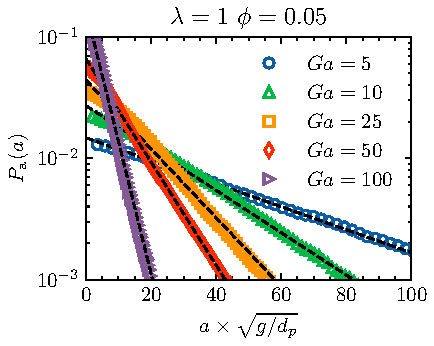
\includegraphics[height = 0.3\textwidth]{image/HOMOGENEOUS_NEW/Dist/Pa_l_1_PHI_5.pdf}
    % 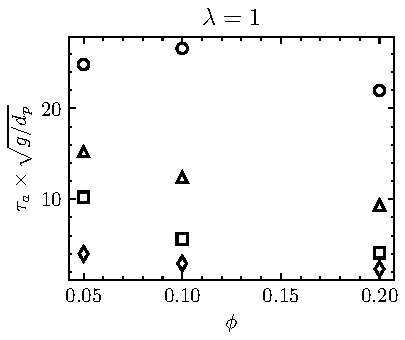
\includegraphics[height = 0.3\textwidth]{image/HOMOGENEOUS_NEW/tau_PHI_l_1.pdf}

    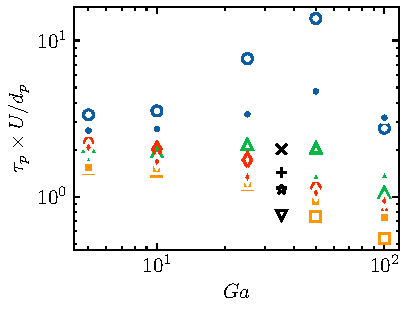
\includegraphics[height = 0.3\textwidth]{image/HOMOGENEOUS_NEW/tau_Ga.pdf}
    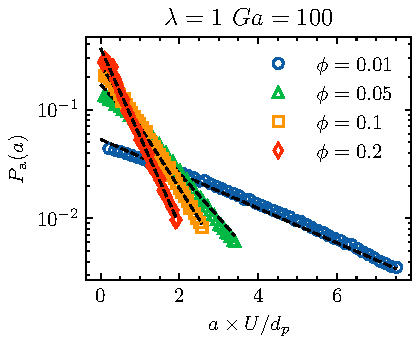
\includegraphics[height = 0.3\textwidth]{image/HOMOGENEOUS_NEW/Dist/Pa_l_1_Ga_100.pdf}
    \caption{
    (left) Mean dimensionless age $\tau_a =  \int_0^\infty aP_a(a)da$ in terms of the \textit{Galileo} number for different volume fraction :   
    ($\pmb\bigcirc$) $\phi = 0.01$; ($\pmb\triangle$) $ \phi = 0.05$; ($\pmb\square$) $\phi = 0.1$ ($\pmb\lozenge$) $\phi = 0.2$.
    The hollow symbols correspond to $\lambda = 1$, the filled symbols to $\lambda = 10$.
    (right) Age distribution function $P_a(a)$ in terms of the dimensionless age, for $\lambda = 1$ and  $Ga = 100$.
    (dashed lines) Theoretical age distribution, $P_a(\textbf{x},t, a) =e^{-a/\tau_p}/\tau_p$ see \ref{eq:Pa}. 
    Both the age and the mean age $\tau_a$ are made dimensionless with the drift velocity $U$ and the particle length scale $d_p$.  
    Black symbols represent the DNS results of \citet{zhang2023evolution} for hard sphere suspension with $\phi = 0.0168,0.0565,0.1341,0.2622$ correspondineg to $\pmb\times, \pmb +, \pmb\star , \pmb\triangledown$, respectively.
    }
    \label{fig:age_picture}
\end{figure}
In \ref{ap:age}  we displayed these same distribution but for $Ga = 10$. 
It is seen that the age distribution for low $\phi = 0.01$ exhibit a higher density for low ages and less for higher age compared to the random distribution.
Therefore, at low \textit{Galileo} and low $\phi$ the \textit{random destruction assumption} doesn't seem to remain valid anymore. 
The \textit{random destruction assumption}  must hold true for flow with high particle velocity fluctuation compared with the mean slip velocity, which induce randomness in particles interaction\citep{zhang2023evolution}.
It is clear that for $\phi \rightarrow 0$ the particle phase fluctuation, also tends to $0$, making this condition false. 
Apart from these two case it is reasonable to say that \ref{eq:Pa} is well representative of the age distribution function. 

In \ref{fig:age_picture} (left) we displayed the dimensionless mean age for all our numerical experiment. 
We can see that for almost all of our DNS, the time of interaction is longer for $\lambda = 1$ and decrease as the \textit{Galileo} number increase. 
The trends with the volume fraction seem constant meaning that it is well scaled with the length scale $d_p$. 
We can see that clearly reaches a peak for $\phi=0.01$, $Ga=50$, $\lambda=1$ which might be correlated with the values of $A_{xx}$ on \ref{fig:A} which also reach a maximum. 
If it is not due to a pure random effect it would mean that since $A_{xx} >0$ particles are in average side-by-side, which means that they might be stable within this configuration, which ultimately implies a large time of interaction.  
The dilute suspension of hard sphere represented by a $\pmb\times$ symbols doesn't seem to follow this trends, as the age remain reasonably low. 
It implies that solid particles doesn't necessarily reach an equilibrium side-by-side configuration in the dilute regime these \textit{Galileo} numbers. 
This might be explained by the generation of more vorticity in the wake of solid particles (in opposition to $\lambda = 1$ cases) which make the interactions unstable at these $Ga$ and $\phi$. 

\subsection{Particle pairs' approach velocity}

In the next section we will be interested in the velocity fields $\textbf{w}_p^\text{nst}$ conditioned on the relative position, since its first moment in \textbf{r} is at the origin of the modifications of the microstructure through the source term \textbf{W} in \ref{eq:dt_R}. 
To give a simpler representation of the relative velocity, we first study the normal approach velocity averaged on all \textbf{r}'s conditioned on the age of the interaction, that is,  
\begin{equation*}
    w_{pn}^a (a)P_a(a)
    = \frac{1}{n_p(\textbf{x},t)}
    \int_{\mathbb{R}^3}
    \textbf{r} \cdot \textbf{w}^\text{nst}_p
    P_\text{nst}(\textbf{x},\textbf{r},t,a) d\textbf{r}.
\end{equation*}
On \ref{fig:normal_vel_picture} (right) we display graphical representation of what we called the normal approach velocity $w_{pn}^a$. 
In this way, $w^\text{a}_n(a)$ is the average relative normal approach velocity between the nearest pair of particles at age $a$. 
It describes the average approach velocity from one particle to its nearest neighbor from the time particles became nearest neighbor, in an averaged sense. 
\begin{figure}[h!]
    \centering
    % 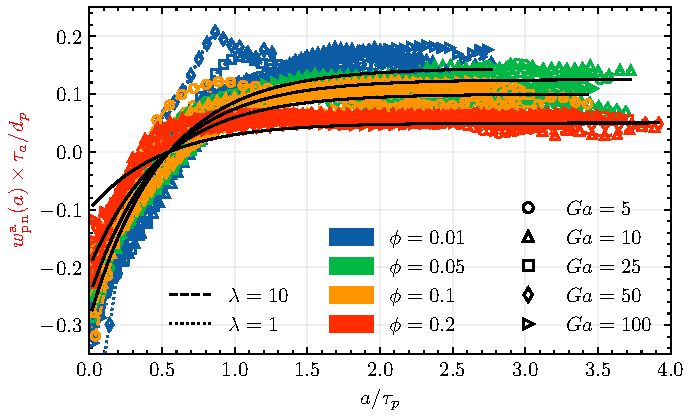
\includegraphics[height = 0.4\textwidth]{image/HOMOGENEOUS_NEW/Age_cond/uR_rel.pdf}
    % \includegraphics[height = 0.3\textwidth]{image/HOMOGENEOUS_NEW/Age_cond/r_l_10_PHI_10.pdf}
    \begin{tikzpicture}[ scale = 0.9]
        \node (img) at (-0.45\textwidth,0){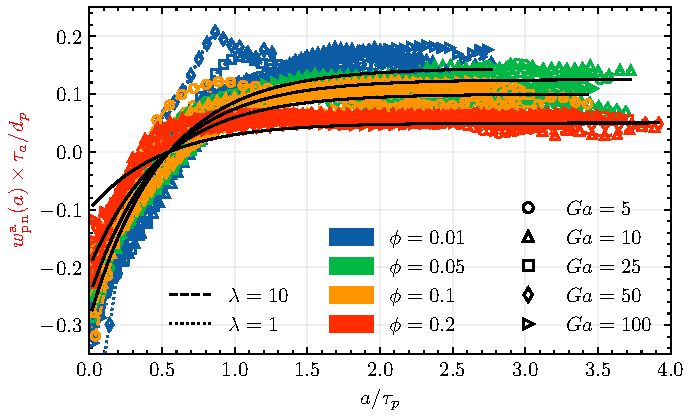
\includegraphics[height = 0.4\textwidth]{image/HOMOGENEOUS_NEW/Age_cond/uR_rel.pdf}};
        \filldraw[ gray!50!white](0,0) circle (0.5)node[left]{$\textbf{x}_i$};
        \filldraw[ gray!50!white](1,3)circle (0.5);
        % \draw[fill=gray,opacity=0.2](5,-0.2)circle (0.5);
        % \draw[fill=gray,opacity=0.2](-3,2)circle (0.5);
        % \draw[fill=gray,opacity=0.2](-5,0.2)circle (0.5);
        \draw(0,0)node[right]{$\textbf{x}_i$};
        \draw[dashed](0,0)--(1,3)node[right]{$\textbf{x}_j = \textbf{x}_i+\textbf{r}(a)$};
        % \draw[very thick,<-,blue](-1,0)--++(0,1)node[right]{$\bm{b}$};
        \draw[very thick,->](1,3)--++(0.9,-1.8)node[above right]{$\textbf{w}^\text{nst}(a)$};
        \draw[very thick,->,red](1,3)--++(-0.5,-1.5)node[left]{$w^\text{nst}_n(a)$};
        \draw[dashed](1,3)++(0.9,-1.8) -- (1,3)++(-0.5,-1.5);
        \node (ii) at (1,-1){$\textbf{w}^\text{nst} = \textbf{u}_j - \textbf{u}_i$};
        \node (ii) at (1,-1.5){$w^\text{nst}_n = \textbf{w}^\text{nst}\cdot \textbf{r}/|\textbf{r}|$};
        % \draw[very thick,->](0,0)--++(1,0)node[below right]{$\bm{e_x}$};
        % \draw[very thick,->](0,0)--++(0,1)node[left]{$\bm{e_y}$};
        % \draw(3,1)++(199:1)node[above left]{$\beta$} arc(199:159:1);
        % \draw(0,0)++(0:1)node[above right]{$\theta$} arc(0:20:1);
    \end{tikzpicture} 
    \caption{(left) Relative normal approach velocity between two nearest neighbors, averaged conditionally on the age of interaction.  
    The age, $a/\tau_a$ as well as the velocity are made dimensionless  with the mean age $\tau_a$ and the length scale $d_p = n_p^{-1/3}$. 
    The symbols represent the different \textit{Galileo} numbers,
    ($\pmb\bigcirc$) $Ga=10$; ($\pmb\triangle$) $ Ga = 25$; ($\pmb\square$) $Ga = 50$ ($\pmb\lozenge$) $Ga =100$.
    The colors represent the different volume fractions, (blue) $\phi =0.01$, (green) $\phi = 0.05$ (organ) $\phi=0.1$ (red) $\phi = 0.2$. 
    The white symbols correspond to $\lambda = 1$, and black symbols to $\lambda = 10$. 
    (colored dashed lines) $\lambda = 1$. 
    (black dashed lines) $a/\tau_a =1$. 
    We observe that all velocity scales with $d_p$ and $\tau_a$. 
    (right)
    Scheme of two nearest neighbors with their position $\textbf{x}_i$ and $\textbf{x}_j$, velocities $\textbf{u}_{i}$ and $\textbf{u}_j$, relative velocity $\textbf{w}^\text{nst}$ and normal relative velocity $\textbf{w}^\text{nst}_n$. 
    }
    \label{fig:normal_vel_picture}
\end{figure}
In \ref{fig:normal_vel_picture}(left) display the approach velocity $\textbf{w}_{pn}^a$ for all the DNS carried in this work. 
The x-axis is scaled with the averaged time of interaction and the y-axis is scaled with the velocity scale $d_p /\tau_p$. 
At  early age $\textbf{w}_{pn}^a<0$, then it eventually reaches zero after what $\textbf{w}_{pn}^a>0$ and is constant in terms of $a$. 
Therefore, in average the particles get closer to each other at early ages, since $\textbf{w}_{pn}^a<0$, then particles get apart at a time $a \gtrapprox \tau_p$, with an averaged constant velocity. 
Two other important features are identified :
(1) The first striking results is that all curves  are roughly similar, even if we can see differences for the different cases with various volume fraction. 
This means that regardless of the flow parameters, $\textbf{w}_{pn}^a$ will scale roughly as $d_p /\tau_p$. 
(2) Second, the velocity stabilize to a constant value at an age $a = \tau_p$. 
Therefore, it seems that $\tau_p$ is also the relaxation time for the particles' relative normal approach. 

Therefore, we demonstrated that $\tau_p$ and $d_p$ were the correct time and length scale which govern the inter particle scale kinematic. 
It is clear that all nearest averaged property will be also subject to a relaxation time $\tau_p$, this in fact comes from the structure of the nearest particle averaged probability transport equation (\ref{eq:dt_Pnst}) which makes appear this relaxation time. 
For now, it is too early to build models based on such relative kinematic behavior, nevertheless this framework might be helpful in future studies to model any averaged term based on interactions. 

